%Background body
%Created MB 04-12

\section{Background}\label{background}

The $^4$He atom is one of the very simple and symmetrical systems
among the elements, with a filled innermost electron shell and no
overall electric or magnetic moment or angular momentum to the atom
\cite{atkins}. Due to the symmetric nature of helium atoms, the
interaction between them is very weak, and $^4$He liquifies at an
extremely low temperature of $4.21$ K. However, a more interesting
transition occurs at $2.17$ K, at which point liquid helium takes on
several unique properties. Below this temperature, termed the
$\lambda$ point, $^4$He\footnote{Although the isotope $^3$He is also
  capable of producing these effects, the transition temperature is
  much lower at $3\times 10^{-3}$ K and is unreachable with the
  cryogenic technology available to us. Thus, in the remainder of the
  paper, the isotope $^4$He is implied unless stated otherwise.}
acquires extremely high thermal conductivity, negligible viscocity,
and the ability to propagate temperature waves(second sound); in
addition, there is a $\lambda$-shaped discontinuity at the transition
in the heat capacity of liquid helium, which is how the $\lambda$
point acquires its name. To distinguish the two phases of liquid
helium, the liquid is referred to as helium I above the lambda point
and helium II below the lambda point (BLAHHH). The investigation of
the properties of helium II mentioned above will be the focus of this
paper.

\subsection{The Two-Fluid Model}

A key model explaining the unusual properties of He II was proposed by
Landau in 1941 as the two-fluid model \cite{landau}. In this theory,
the liquid below the $\lambda$-point can be viewed as being composed
of two noninteracting fluids: a superfluid component with density
$\rho_s$ and a normal component with density $\rho_n$, such that the
total density $\rho$ is given as the sum of the two components:
\begin{equation}
\rho = \rho_s + \rho_n
\end{equation}

and the total current density of He II is given by
\begin{equation}
\mathbf{j} = \rho_s\mathbf{v_s} + \rho_n\mathbf{v_n}
\end{equation}

where $\mathbf{v_s}$ and $\mathbf{v_n}$ are the velocities of the
superfluid and normal fluid, respectively \cite{tilley}. Then, the
behavior of the fluid can be understood in terms of the different
characteristic of the two components: while the normal fluid acts
according to the regular laws of fluid mechanics and satisfies the
Navier-Stokes equation, the superfluid has zero entropy and flows with
zero viscocity. Furthermore, it is important to note that the two
components are non-interacting, that is, there is no transfer of
momentum between the two fluids, and most importantly that they are
not physically distinct and cannot be separated \cite{tilley}.

With the incorporation of theories of Bose-Einstein condensates into
Landau's theory, further understanding of the fluid is possible. The
superfluid can be viewed as an interacting Bose-Einstein condensate
system, occupying a single macroscopic quantum state, whereas the
normal fluid consists the excitations (photons and rotons) of the
superfluid. As temperature decreases from $2.17$ to $0$ K, the
fraction of superfluid increases, from $0$ at the $\lambda$-point to
unity at absolute zero, as the excitations decrease to zero.

\begin{figure}[ht]
\begin{center}
\input{./figures/twofluid.eps}
%\caption{\small{Test}}
%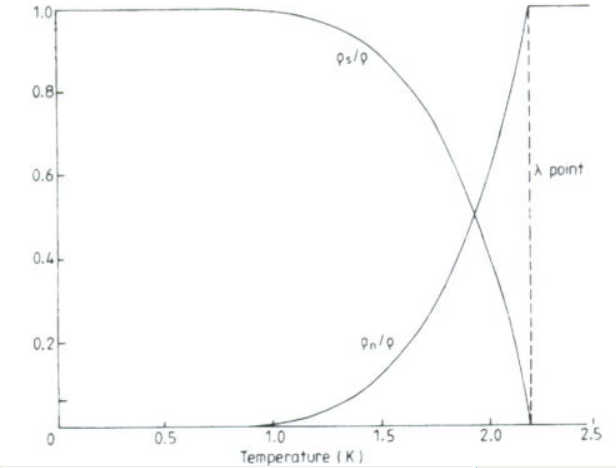
\includegraphics{./figures/twofluid.eps} WHY NOT WORKINGGGGGGG
%\{./figures/twofluid.eps}
\caption{\small{Relative fractions $\rho_s/\rho$ and $\rho_n/\rho$ of
    the superfluid and normal components in He II.}}
\label{figure:twofluid}
\end{center}
\end{figure}



\subsection{Second Sound}

The thermal conductivity of He II is very high, and tends to infinity
for small heat currents \cite{tilley}. This makes the fluid intolerant
to temperature gradients. This property explains the visually
noticeable transition from He I to He II with descreasing temperature:
while in He I, there is a lot of bubbling, as the temperature passes
the $\lambda$-point, the bubbling ceases immediately, since a
temperature gradient large enough cannot be established in order for a
bubble to form \cite{tilley}.

Interestingly, the superfluid fraction cannot transfer heat, but is
able to balance temperature gradients not through convection and
BLAHHOTHERTHING but through an exchange of the relative concentrations
of the two componenets $\rho_n$ and $\rho_s$. As seen in FIGURE
TWOFLUID, at lower temperatures the fraction of superfluid increases.

The relationship between velocity of second sound, $u_2$, and the
relative fractions of the fluids was derived analytically by Landau
and is given by

\begin{equation}
u_2^2 = \frac{\rho_s}{\rho_n}\frac{T S^2}{C}
\end{equation}

where $S$ and $C$ are the entropy and heat capacity per gram of the
liquid and can be measured experimentally \cite{atkins}. 

\subsection{Heat Capacity}
